\documentclass[12pt]{article}

\usepackage{scicite,times,graphicx,float,hyperref}
\usepackage[skip=0pt]{caption}

\topmargin -1.0cm
\oddsidemargin 0.0cm
\textwidth 16cm 
\textheight 23cm
\footskip 1.0cm

\newenvironment{sciabstract}{%
\begin{quote} \bf}
{\end{quote}}

\newcounter{lastnote}
\newenvironment{scilastnote}{%
  \setcounter{lastnote}{\value{enumiv}}%
  \addtocounter{lastnote}{+1}%
  \begin{list}%
  {\arabic{lastnote}.}
  {\setlength{\leftmargin}{.22in}}
  {\setlength{\labelsep}{.5em}}
}
{\end{list}}

\title{Lab Work 2} 

\author
{André Pedrosa [85098], Filipe Pires [85122], João Alegria [85048]\\
\\
Algorithmic Information Theory\\
\normalsize{Department of Electronics, Telecommunications and Informatics}\\
\normalsize{University of Aveiro}\\
} 

\date{\today{}}

%%%%%%%%%%%%%%%%% END OF PREAMBLE %%%%%%%%%%%%%%%%

\begin{document} 

\baselineskip18pt

\maketitle 

\section*{Introduction}

This report aims to describe the work developed for the second assignment
of the course of 'Algorithmic Information Theory', explaining all programs
developed by us, and presenting the results we considered most relevant 
regarding the quality of the solutions. 

The programs implemented in C++ have the purpose of analysing and encoding
audio files and ultimately being capable of, from a small audio segment, 
identifying the music that it most likely belongs to.

Along with the description of the solution, we also discuss the effects
of the variation of the programs' parameters and how accurate are the results.
All code developed is publicly accessible in our GitHub repository:
\url{https://github.com/joao-alegria/TAI} .
\newpage

\section*{1. Data Visualization}

In this chapter we present a description of the dataset used, the small script 
we developed to convert audio segments from stereo to mono and the histograms
we are capable of plotting by adapting one of the scripts given along with the
assignment's description \cite{trab1}.

\subsection*{1.1. Dataset}

We were given the access to a small dataset containing 7 audio files from 
different musics. It was these music fragments we used to test our code during 
development.
Each audio file is in \texttt{.wav} format and has two signal channels (stereo).
They vary between 13 and 29 seconds of audio and, when played, none seems to 
contain significant noise.

For testing the performance of the programs once the development phase was
completed, we came up with our own dataset of musics of different genres.
These music files vary between 3:07 and 8:09 minutes and have the same format 
and number of channels as the original dataset.
As they were downloaded from the original sources, their quality is close to 
ideal.

\subsection*{1.2. Mono Conversion}

One of the tasks proposed was to create a script that converts stereo audio 
files into mono.
This was fairly straightforward to do, as it only required for us to read the v
alues from all signal channels and calculate the average of each.
The script is executed in the format presented below, once built:

\begingroup
\addtolength\leftmargini{-0.4in}
\begin{quote}
\begin{verbatim}
$ ./wavquant inputFile outputFile [-q quantSize] [-r reductFactor]
\end{verbatim}
\end{quote}
\endgroup

This script, \texttt{wavquant.cpp}, is also used for other purposes, in which 
the \texttt{quantSize} and \texttt{reductFactor} parameters are useful.
For this reason, we made the parameters optional, so that a user can run 
\texttt{wavquant} to simply convert stereo files into mono, with a default 
number of bits used to encode each value of the segment (each sample) of 16 and 
no frequency reduction factor.
This script is mentioned further ahead in greater detail.

\subsection*{1.3. Histograms}

We were also given a script called \texttt{wavhist.cpp} that outputted to the 
terminal the histogram of an audio file.
We adapted this script so that it accepts both stereo and mono audio files 
and plots in a figure the histogram of one of the audio channels.
The script uses \texttt{gnuplot} \cite{gnuplot}, a portable command-line driven 
graphing utility, and has the following format:

\begingroup
\addtolength\leftmargini{-0.4in}
\begin{quote}
\begin{verbatim}
$ ./wavhist inputFile channel
\end{verbatim}
\end{quote}
\endgroup

Figures \ref{fig:histogram_stereo} and \ref{fig:histogram_mono} contain the 
histograms plotted from the same music in the original format (stereo) and after 
its conversion to mono. 
The x axis represents the frequency of the values and the y axis the number of 
occurences in the music of each frequency.

\begin{figure}[H]
  \centering
  \begin{minipage}{.5\textwidth}
    \centering
    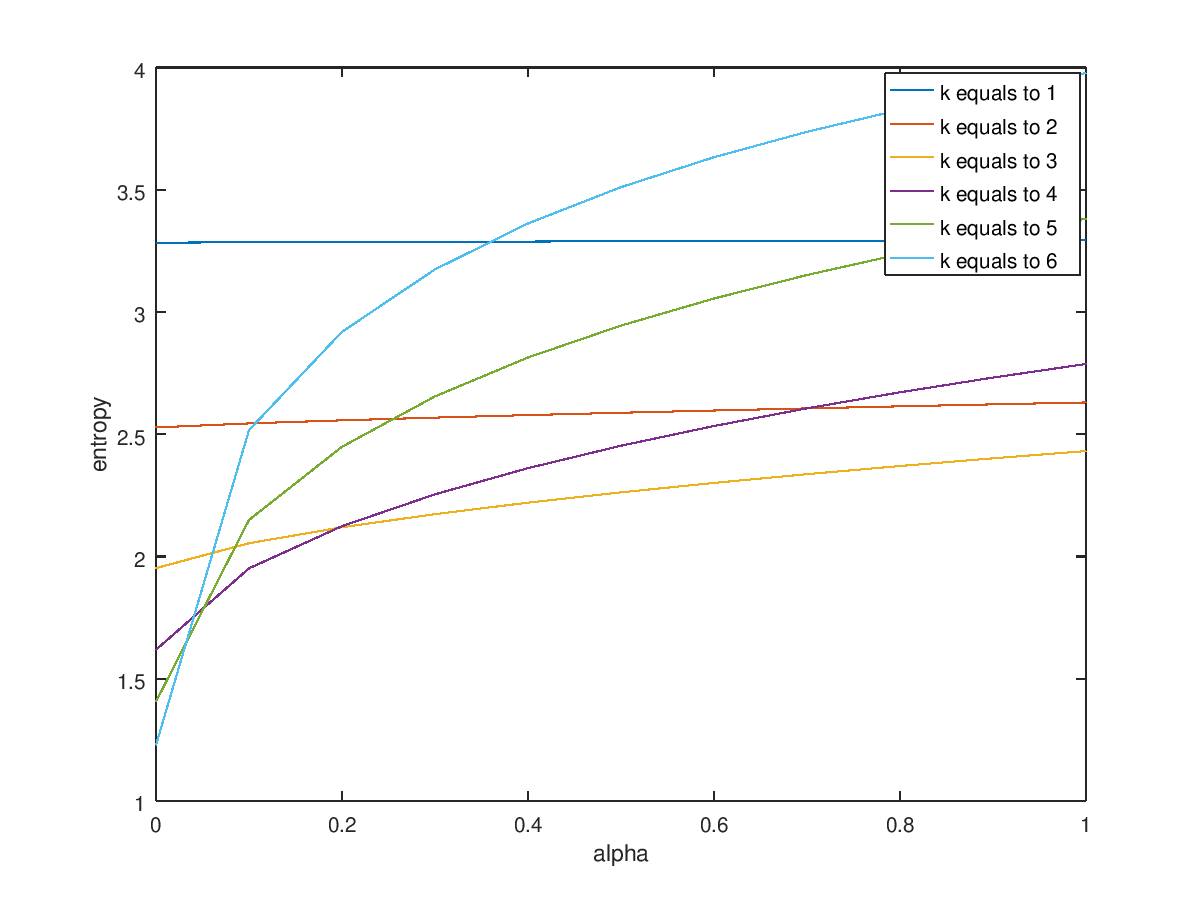
\includegraphics[width=\linewidth]{bible_en.png}
  \end{minipage}%
  \begin{minipage}{.5\textwidth}
    \centering
    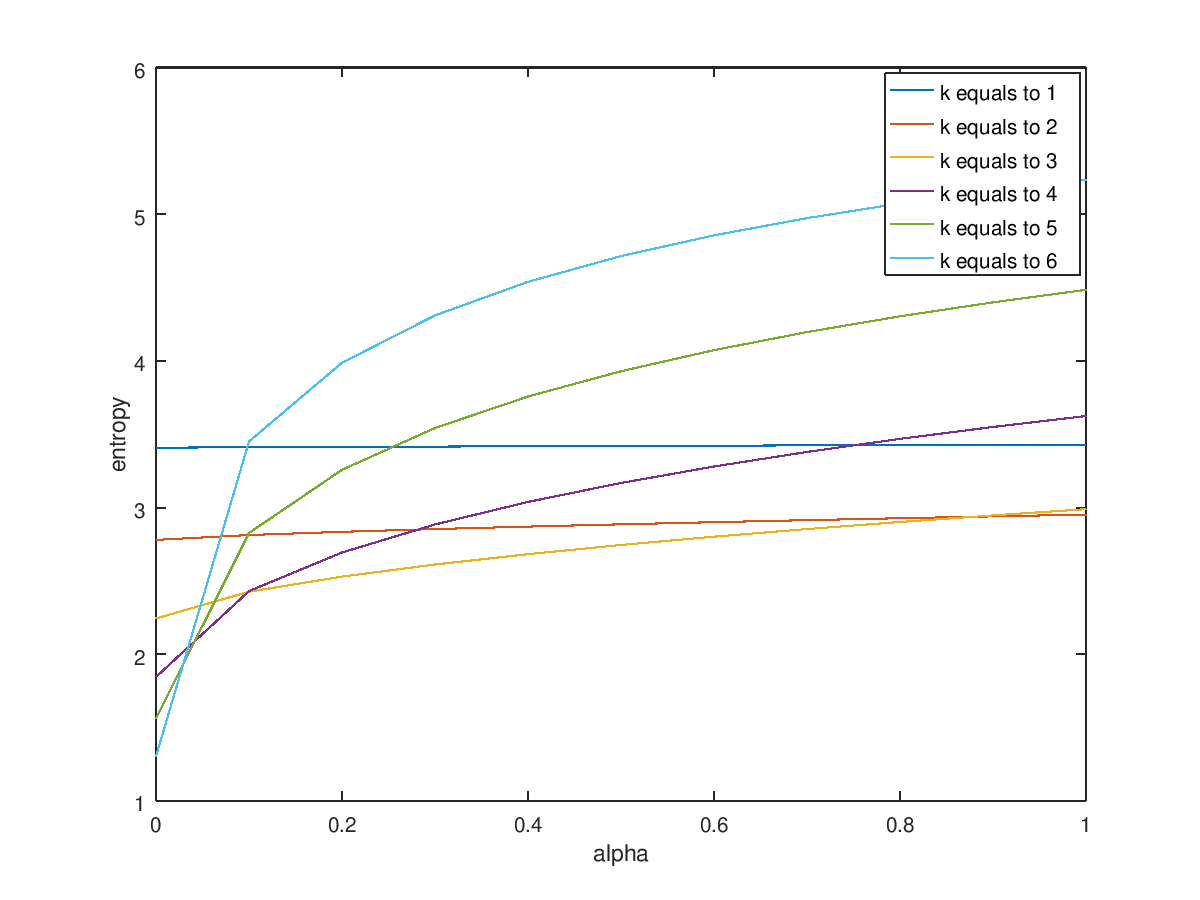
\includegraphics[width=\linewidth]{bible_pt.png}
  \end{minipage}
  \caption{Histogram of music\_name in the original format - channels 0 and 1.}
  \label{fig:histogram_stereo}
  
  \centering
  \begin{minipage}{.5\textwidth}
    \centering
    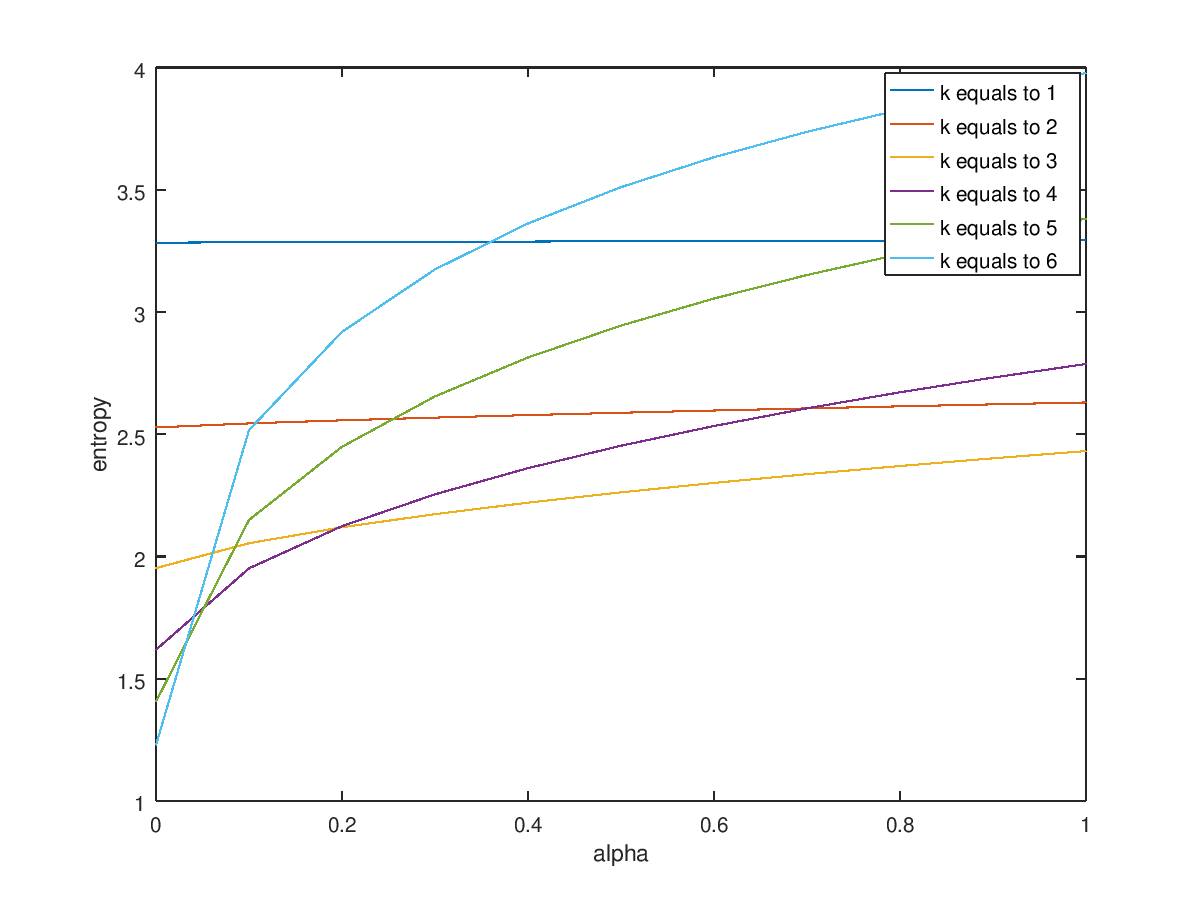
\includegraphics[width=\linewidth]{bible_en.png}
  \end{minipage}%
  \caption{{Histogram of music\_name after its conversion to mono (1 channel only).}}
  \label{fig:histogram_mono}
\end{figure}

............

Mention something about why do the shapes are as they are and why is mono so different

............

The C++ scripts mentioned in this chapter all use \texttt{libsndfile}, a C 
library used for reading and writing files containing sampled sound \cite{libsndfile}.
This was proposed on the assignment and allowed us to read and manipulate the 
audio files for more complex tasks.

\newpage
\section*{2. Data Processing}

Once we were capable of visualizing the data, we proceeded to actually doing 
something useful with it.
In this chapter we explain the implementation of the program \texttt{wavquant.cpp},
responsible for reducing the number of bits used to represent each audio sample.
The implementation of the formulas presented on the assignment's description for
the signal-to-noise ratio and the energies of the signals and noises is described
as well, along with the computation of vector quantization codebooks of audio files.

\subsection*{2.1. Uniform Scalar Quantization}

The idea behind a uniform scalar quantization (USQ) is the reduction of bits 
used to represent a signal.
Its usage has an instrinsic tradeoff between signal quality and memory space
required to store the information.
We do not get into much detail regarding the mathematics behind this process, 
but we make available a figure taken from a presentation from the Stanford 
University \cite{stanford} that helps visualizing the outcome of applying the 
USQ to a signal.
Figure \ref{fig:quantization} contains a signal presented in blue and the outcome
of the signal after it is quantized is presented in red. 
The figure also contains the quantization error variation on
the second plot.

\begin{figure}[H]
  \centering
  \begin{minipage}{\textwidth}
    \centering
    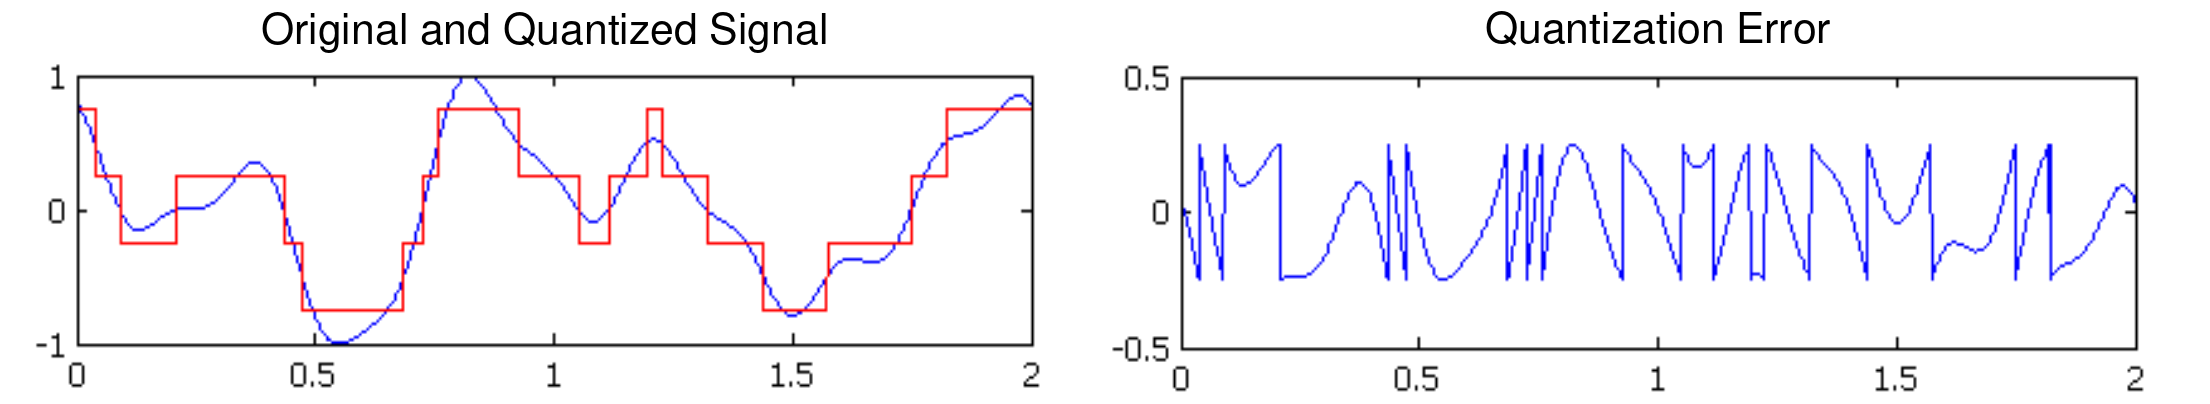
\includegraphics[width=\linewidth]{stanford_quantization_wide.png}
  \end{minipage}%
  \caption{Example of a quantized waveform.}
  \label{fig:quantization}
\end{figure}

It is \texttt{wavquant.cpp} that is responsible for this process.
As we have seen in Section 1.2, the script accepts two optional parameters:
\texttt{quantSize} defines the number of bits to be used to represent the audio 
fragment given as input (ideally, this value should be less than of the original 
source); \texttt{reductFactor} defines the number of times the user would like 
to reduce the total number of values of the audio signal.
This reduction factor works by calculating the average between \texttt{n} values, 
where \texttt{n = reductFactor}, and doing this for all values from the segment.
The result is a signal with \texttt{n} times less values (samples).

\newpage
\subsection*{2.2. Error Calculation}

A signal-to-noise (SNR) ratio compares a level of signal power to a level of 
noise power. 
Higher numbers generally mean a better specification, since there is more useful 
information (the signal) than there is unwanted data (the noise).

In \texttt{wavcb.cpp} we calculate this ratio, along with the maximum absolute 
error per sample. The SNR is defined as stated in equation \ref{eq:1}, taken 
from the assignment's description.

\begin{equation} \label{eq:1}
  SNR = 10 log_{10} \frac{E_{s}}{E_{n}} (dB)
\end{equation}

Here, $E_s$ is the energy of the signal, given by $E_s = \sum_{k} x_k^2$, and
$E_n$ is the energy of the noise, given by $E_n = \sum_{k} (x_k-\bar{x}_k)^2$,
where $x$ is the values from the audio segment.
The maximum error is defined in equation \ref{eq:2}, derived from the noise 
energy equation.

\begin{equation} \label{eq:2}
  error = |x_k-\bar{x}_k| \Leftrightarrow 
  max(error) = max(|x_k-\bar{x}_k|)
\end{equation}

In practice, the error of a quantization tells us how distant from the original
signal is the quantized one.
Figure \ref{fig:quantization} shows an example of how this error looks like.

However, for the following assignment tasks, we determined that the energy of
the noise would be more useful to us.
One way to compare audio fragments would be through the signal-to-noise ratios;
But we found that the only calculations actually required are of the noise 
energies as they work as the distances between two samples.
By focusing on these values, not only do we save processing time, but we are
also able to compare input audio segments to quantization codebooks already 
present in a program to determine the similarity between samples (and 
consequently between segments). These codebooks are explained in this next section.

\subsection*{2.3. Vector Quantization Codebook}
\label{sec:vctQuantCB}

Each music from the datasets is represented as a sequence of samples, where each 
sample is a singular frequency (if the file is in mono) or the pair of frequencies 
(one per channel, if the file is in stereo) that was registered in that exact second.
What a codebook is is basically an abstract representation of the overall 
sequence of samples.

In the context of our project, we integrated the concept of clusters to represent 
a given number of samples.
The base idea of this clustering is that similar data entities should have similar 
properties and can therefore be aggregated in a group.
On the other hand, data entries that differ significantly from each other
have properties considerably different as well, implying that they should belong 
to different groups \cite{clustering}. 

\newpage
Dividing the totality of samples present in each music into vectors with 'x' 
samples and representing them as points in a multidimensional vectorial space -  
as seen in Figure \ref{fig:pointsEx} - enables us to better comprehend the 
structure of the clusters.  
Geometrically speaking, clusters can be directly identified by the close 
grouping of the multidimensional points, since each axis represents a data 
property and similar points with similar properties stay closer to each other. 

By taking advantage of this natural grouping, clustering algorithms try to find 
points that represent the several data groups in a useful way, usually 
corresponding to the middle point of each group, known as centroid.

\begin{figure}[H]
  \centering
  \begin{minipage}{\textwidth}
    \centering
    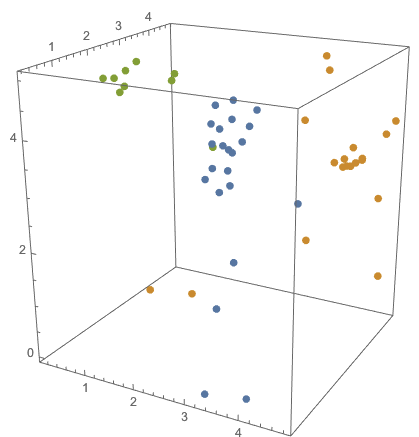
\includegraphics[width=0.4\linewidth]{pointsEx.png}
  \end{minipage}%
  \caption{Example of a 3-D visualization of point clusters.}
  \label{fig:pointsEx}
\end{figure}

So, in short, our interest in using such algorithms lies in the applicability of 
converting audio files into multidimensional clusters so that the most likely
cluster a new audio segment belongs to can be more easily identified.
A codebook is defined by the clusters that resulted from the process of mapping
the input audio file to its multidimensions.

In our implementation we used the K-Means Clustering algorithm, one of the 
most well-known clustering algorithm \cite{clustering}. 
K-Means was considered a good approach because it is relatively simple to 
implement and fast to execute, as it only requires the calculation of the 
distance between a given point and all existing centroids. 

The way it works is as follows.
The code starts by doing the already mentioned music partition in different 
blocks/vectors of a given size provided by the user;
Then the algorithm chooses, in a random fashion, an number of centroids given 
{\it a priori\/};
Once the pre-processing is done, the main algorithm begins calculating the 
closest centroid for each vector, and then updates each centroid by calculating 
the middle point of the points assigned to that specific centroid - this is 
repeated as many times as necessary for the error delta, i.e. the error between 
each iteration, to be lower than a given threshold specified by the user. 

The script \texttt{wavcb.cpp} is the implementation of this algorithm.
It enables the creation of a codebook for a given music by following the format 
below:

\begingroup
\addtolength\leftmargini{-0.4in}
\begin{quote}
\begin{verbatim}
$ ./wavcb inputFile blockSize overlapFactor errorThreshold
  numRuns outputFile
\end{verbatim}
\end{quote}
\endgroup

{\it InputFile\/} is the path to the .wav music whose codebook is to be constructed.
{\it BlockSize\/} is the value used as the size (number of samples) of the blocks 
in which the audio file is split.
{\it OverlapFactor\/} corresponds to the factor (a value between 0 and 1) that 
each block will be overlapped with the previous block; the bigger the overlapping
percentage is, the better the music is represented in the multidimensional space.
{\it CodebookDir\/} is the path to the directory containing the 
preprocessed codebooks of the music dataset.
{\it ErrorThreshold\/} is the maximum error that is allowed to exist in the last 
iteration; below this threshold, the centroids are no longer being adjusted in a 
worthwhile manner.
{\it NumRuns\/} is the number of times the K-Means algorithm will run to find 
the best local minimum; each run is initialized with the centroids in different 
positions.
At last, {\it outputFile\/} is the path to the file were the codebook will be stored. \\

Although quite flexible, K-Means has some disadvantages.
The most significant to our needs are the fact that it is necessary to insert the 
number of centroids to take in consideration which, in many situations, is not 
the best option, since the main purpose of using clustering is to get some 
insights about the data, preferring that the algorithm finds the number of 
centroids by itself; also, as K-Means' centroids start from a random starting 
position that is different each time it is executed, this makes it non-deterministic
and therefore not optimal as it can converge into a local minimum.
This last issue is dealt with in our solution by running K-Means several times to 
gain access to several local minimums and then choose the best one. 
As it is stated above, the number of times it is executed is defined by {\it numRuns\/}.

\newpage
\subsection*{2.4. Codebook Parallel Processing}

As audio files get longer, the number of frames per file increases and 
consequently so does the number of blocks that will be extracted from them.
Furthermore there is the overlapping factor detail, which increases even more 
the total number of blocks.
This high number of blocks brings computational time implications since, on the 
blocks classification step of the K-Means algorithm, each centroid has to be 
compared with each block and the closest centroid for each block must be determined.

Even though K-Means is considered a fast clustering algorithm, if given a 
considerable number of data entries, it is understandable that it starts to 
become cumbersome. 
To deal with this effect, we introduced parallelism into the process.
Practically speaking this means that we divide the blocks into groups and create
threads responsible for them and the calculation of the closest centroid.
To prevent having to create complex synchronization mechanisms, each thread 
stores the association between blocks and the closest centroids on different 
data structures and then the main thread is in charge of reading from those to 
recalculate the centroids.

As mentioned in the previous section, we deal with one of the K-Means algorithm's
disadvantages by testing it several times with different centroid initializations.
It is needless to say that this also slows down the algorithm.
To ease this, each K-Means run can be assigned to a thread, allowing to execute 
several runs at the same time.
In terms of implementation it implies some synchronization mechanisms, so the 
main thread knows when a run was completed and to manipulate the structure to 
store the centroids plus the associated error calculated on each run.

Figure \ref{fig:threading} is a visual representation of the execution flow of 
generating a codebook. 
The two independent time axis correspond to executing without additional threads 
and with 2 threads in each parallelization point.
Note that this is not an exact time representation and is ment only to illustrate
the advantage of multithreading. 

\begin{figure}[H]
  \centering
  \begin{minipage}{\textwidth}
    \centering
    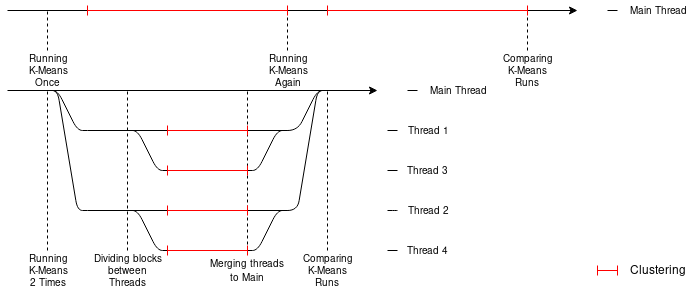
\includegraphics[width=0.95\linewidth]{threading.png}
  \end{minipage}%
  \caption{Visual representation of the execution flows with and without threading.}
  \label{fig:threading}
\end{figure}

\newpage
\section*{3. Automatic Music Identification}

The program \texttt{wavfind.cpp} is the application of the previous scripts on a 
program with a specific purpose.
WAVFind is ment to interpret an audio fragment and attempt to identify which music 
from a database it belongs to.
In this chapter we discuss our solution, the consequences of varying the 
parameters passed to it and the quality of the results.

\subsection*{3.1. Most Probable Music}

The idea of WAVFind is very similar to the well known mobile app Shazam 
\cite{shazam} - a user plays a sound, the app listens to it, processes it and
determines the most probable music that sound belongs to.
Shazam has a large infrastructure, counting on online real-time music detection,
a nice user interface with access to the smartphone's microphone, and a variety
of other features.
We, on the other hand, focus on the functional end of this idea, implementing
it as a command line program with a limited dataset of known musics and with
the capacity to receive audio segments as input through their respective paths 
on the computer running the command.

To execute this command, one needs to use the following format:

\begingroup
\addtolength\leftmargini{-0.4in}
\begin{quote}
\begin{verbatim}
$ ./wavfind inputFile blockSize overlapFactor codebookDir
\end{verbatim}
\end{quote}
\endgroup

All arguments are mandatory and most of them we have seen on previous commands. 
{\it InputFile\/} is the path to the .wav audio whose origin music is to be identified.
{\it BlockSize\/} is the value used as the size of the blocks in which the audio 
segment is split; this value must be the same size used when the codebooks of 
the music dataset were built.
{\it OverlapFactor\/} corresponds to the factor (a value between 0 and 1) that 
each block will be overlapped with the previous block.
At last, {\it codebookDir\/} is the path to the directory containing the 
preprocessed codebooks of the music dataset.

The dataflow of the program is as follows:
first, the {\it inputFile\/} is validated and its information is extracted; 
then, it is split into blocks with size according to the parameter {\it blockSize\/}; 
now, for each codebook present in the {\it codebookDir\/}, each segment block 
is compared to each codebook block by calculating the $E_n$ (noise energy) 
between the two;
here, the minimum $E_n$ of each segment block is summed to a cumulative total
that represents the error between the segment and the codebook;
as this cumulative error is calculated for all codebooks, we then check which 
codebook returned the smallest error and assign it as the most similar to the
given audio segment.
This smallest error is determined iteratively - as each codebook is processed, 
we compare its cumulative error to the previous one and keep the smallest.
The identified codebook's is finally printed onto the console (as its name is 
supposed to identify the music it belongs to).

Now, for the program to work properly, there are a few prerequisites.
First of all, the program must have access to the codebook dataset.
The process of creating codebooks is neither trivial nor short-lasting, so to 
have access to the audio dataset is not enough.
Next, the audio segments passed as input files must contain only one signal 
channel (mono).
This restriction reduces the complexity of the comparison process, with the
obvious tradeoff of reducing the quality of the audio.
On the other hand, in a real case scenario (like with Shazam), the user would
usually record audio fragments from external sources such as speakers; so, to 
consider characteristics related to stereo files in the music identification 
process could lead to deceiving the program as the recording could fail in 
distributing the collected information to the proper channels.

\subsection*{3.2. Parameters Variation}

In this section we present some results of executing WAVFind for all datasets.
We also explain some experiences done with variations to the parameters passed
to the command and the respective consequences.

...

\subsection*{3.3. Results Discussion}

...

\newpage
\section*{Conclusions}

After completing the assignment, we drew a few conclusions regarding our 
solutions and the applicability of algorithms such as the K-Means to solving
problems such as music identification.

First of all, ...

Regarding our satisfaction with the delivered code,...

In terms of code organization and readability, we made sure our 
repository was as well structured as possible and our code properly commented
and documented.
The base folder contains a {\it README\/} file for basic instructions and a 
{\it Makefile\/} to make the compilation process easier.
All code is in the {\it src\/} folder and its documentation is accessible, 
with the help of the {\it Makefile\/} and the command "make docs", through
the automatically generated {\it index.html\/} file in the {\it docs\/} 
directory.

\begin{thebibliography}{9}
  \bibliographystyle{Science}

  \bibitem{trab1}
    Armando J. Pinho,
    \textit{AIT: Lab Work no.2},
    University of Aveiro,
    2019/20.
  
  \bibitem{gnuplot}
    H.B. Broeker, G. Clark, L. Hecking and E. Merritt,
    \textit{Gnuplot: graphing utility},
    \url{http://www.gnuplot.info/} ,
    May 2019,
    [accessed in: November 2019].

  \bibitem{libsndfile}
    Free Software Foundation,
    \textit{GLibsndfile API},
    \url{http://www.mega-nerd.com/libsndfile/api.html} ,
    April 2013,
    [accessed in: November 2019].

  \bibitem{stanford}
    Bernd Girod,
    \textit{Image and Video Compression: Quantization},
    \url{https://web.stanford.edu/class/ee398a/handouts/lectures/05-Quantization.pdf} ,
    [accessed in: November 2019].

  \bibitem{shazam}
    Apple Inc.,
    \textit{Shazam for iOS \& Android},
    \url{https://www.shazam.com/apps} ,
    [accessed in: November 2019].

  \bibitem{clustering}
    George Seif,
    \textit{The 5 Clustering Algorithms Data Scientists Need to Know},
    \url{https://towardsdatascience.com/the-5-clustering-algorithms-data-scientists-need-to-know-a36d136ef68} ,
    [accessed in: November 2019].

\end{thebibliography}

\clearpage

\end{document}




















